% % % % % % % % % % % % % % % % % % % % % % % % % % % % % % % % % % % % % % % % 
% LaTeX Cheat Sheet von LaTeX4EI                                                                        
%
% @encode:      UTF-8, tabwidth = 4, newline = LF
% @author:      Emanuel Regnath
% @date:                
%
% % % % % % % % % % % % % % % % % % % % % % % % % % % % % % % % % % % % % % % % 


%---------------------------------------%
%                       P R E A M B L E                         %
%~~~~~~~~~~~~~~~~~~~~~~~~~~~~~~~~~~~~~~~%
% arara: indent: {overwrite: yes, silent: yes}
\PassOptionsToPackage{english}{babel}

% Document Class ===============================================================
\documentclass[fs, footer]{latex4ei}

\usepackage{cprotect}
\usepackage{hyperref}
\usepackage{scientific}

% My packages
\usepackage{makecell}
\usepackage{mathtools}
\usepackage{cleveref}
\usepackage{float}
\usepackage{capt-of}
\usepackage{graphicx}
\graphicspath{{figures/}}

\newcommand*{\vertbar}{\rule[-1ex]{0.5pt}{2.5ex}}
\newcommand*{\horzbar}{\rule[.5ex]{2.5ex}{0.5pt}}

% language
\selectlanguage{english}

%colors
\colorlet{sectioncolor}{tum_blue_dark2}

% Idee: eigene farbe {blue_dark1}, Zuweisungsfarbe {col:section} oder {col:table}
% F�r \code in sectionbox: neue sectionbox als umgebung mit minipage



% Source Code Listings =========================================================
\usepackage{listings}
\definecolor{listinggray}{gray}{0.9}
\definecolor{lbcolor}{rgb}{0.9,0.9,0.9}
\lstset{
    backgroundcolor=\color{lbcolor},
    basicstyle=\tt,
    tabsize=2,
    language={[LaTeX]TeX},
    %upquote=true,
    aboveskip={0.4\baselineskip},
    belowskip={0.4\baselineskip},
    abovecaptionskip={\baselineskip},
    belowcaptionskip={0\baselineskip},
    columns=fixed,
    showstringspaces=false,
    extendedchars=true,
    linewidth=6.7cm,
    xleftmargin={3pt},
    %framexleftmargin={10pt},
    framexrightmargin={2pt},
    %framextopmargin={9pt},
    %framexbottommargin={9pt},
    %breaklines=true,
    prebreak = \raisebox{0ex}[0ex][0ex]{\ensuremath{\hookleftarrow}},
    frame=single,
    showtabs=false,
    showspaces=false,
    showstringspaces=false,
    identifierstyle=\ttfamily,
    %tagstyle=\bf,
    keywordstyle=\color{tum_blue_dark},
    commentstyle=\color[rgb]{0.133,0.545,0.133},
    stringstyle=\color[rgb]{0.8,  0.1,  0.1},
}

\let\myverb\lstinline
\let\code\lstinline
%\renewcommand{\code}[1]{\lstinline?#1?}

\usepackage{fancyvrb} 
\usepackage{verbdef} 
\DefineShortVerb{\#}



\fancyfoot[R]{Created \today \ at \thistime \qquad \thepage}
\fancyfoot[L]{Homepage: \href{www.latex4ei.de}{www.latex4ei.de} -- please report misstakes \emph{immediately}.}
\fancyfoot[C]{by Emanuel Regnath, contact \emph{\href{mailto:emanuel.regnath@tum.de}{emanuel.regnath@tum.de}}}


% Define BibTeX command
\def\BibTeX{{\rm B\kern-.05em{\sc i\kern-.025em b}\kern-.08em T\kern-.1667em\lower.7ex\hbox{E}\kern-.125emX}}


% Hyperref
\hypersetup{
        pdfcreator={LaTeX2e},
        pdfborder=0 0 0,
        breaklinks=true,
        bookmarksopen=true,
        bookmarksnumbered=true,
        linkcolor=tum_blue_dark,
        urlcolor=tum_blue_dark,
        citecolor=tum_blue_dark,
        colorlinks=true
}


% make boxes robust for verbatim
\let\oldsectionbox\sectionbox
\outer\def\sectionbox{\icprotect\oldsectionbox}


%---------------------------------------%
%                       LaTeX Cheat Sheet                       %
%~~~~~~~~~~~~~~~~~~~~~~~~~~~~~~~~~~~~~~~%

% DOCUMENT_BEGIN ===============================================================
\begin{document}

% Split in 4 Columns ===========================================================
\begin{multicols*}{4}

% TITLE ========================================================================
\fstitle{MIT 18.06 Notes \\[0.3em] {\normalfont \small Notes from Dr. Strang's course on linear algebra}}


%{\large Principle: �Write clear \& beautiful english with \textrm{\LaTeX}!�}
% options for environments \tabcolsep
% links to package description in headings
% lstlisting, subfigure
% how to include beautiful matlab plots
% overwiev of important packages:
% multicol, rotate, chem


% SECTION ====================================================================================
\section{Geometry of linear equations}
% ============================================================================================

\sectionbox{
        \subsection{Overview}
        This lecture mainly discusses the three visualization techniques--matrix picture, row picture, and column picture--that are typically used for understanding linear equations, and very briefly touches upon the concepts of linear combination and matrix multiplication.  
}

\sectionbox{
        \subsection{Linear system visualization techniques}
        Dr. Strang proposed the following three visual techniques to understand a linear system of equations before solving them:
        
        \begin{tabular}{@{}ll@{}}\trule
                \textrm{Picture type} & \textrm{Explanation} \\ \mrule
                Matrix picture & \makecell[tl]{It's the algebra way to visualize a linear system using \\ the equation $Ax = b$*} \\
                Row picture & \makecell[tl]{It's the picture created from plotting the solutions to \\ each equation (or row of $A$) in the linear system} \\
                Column picture & \makecell[tl]{It's the picture created from plotting the columns of \\ $A$ and their linear combination that yields $b$} \\ \brule
        \end{tabular}
        *$A$ is the coefficient matrix, $x$ is the vector of unknowns, and $b$ is the right-hand side vector \\

        The subsequent sections show the examples of matrix picture, row picture, and column picture for $2 \times 2$ and $3 \times 3$ system of equations.
}

\sectionbox{
\subsection{2-by-2 equations}
For the first example, consider the following system with two equations in two unknowns,

\begin{equation}
\begin{alignedat}{1}
2x - y &= 0 \\
-x + 2y &= 0 
\end{alignedat}
\label{eq:lec01-2d-case}
\end{equation}        

, and visualize it using matrix picture, row picture, and column picture.
}

\sectionbox{
\subsection{Matrix picture}
To get the matrix picture, express the equations $2x - y = 0$ and $-x + 2y = 3$ in the form $AX = b$:

\[
\begin{bmatrix*}[r]
2 & -1 \\
-1 & 2
\end{bmatrix*}
\begin{bmatrix*}
x \\
y
\end{bmatrix*}
=
\begin{bmatrix*}
0 \\
3
\end{bmatrix*}
\]
}

\sectionbox{
\subsection{Row picture}
To get the row picture, plot all the points that satisfy the equations $2x - y = 0$ and $-x + 2y = 3$:

\begingroup
\centering
\includegraphics[scale = 0.5]{lec01_geometry-of-linear-equations/fig01_2d-row-pic/figure.pdf}
\par
\endgroup
}

\sectionbox{
\subsection{Column picture}
To get the column picture, plot the columns of the coefficient matrix, 
$\begin{bmatrix*}[r]
2 & -1 \\ 
-1 & 2
\end{bmatrix*}$, for the equations $2x - y = 0$ and $-x + 2y = 3$ and combine them in right amounts to get
$\begin{bmatrix*}[r]
0  \\ 
3
\end{bmatrix*}$:

\begingroup
\centering
\includegraphics[scale = 0.5]{lec01_geometry-of-linear-equations/fig02_2d-col-pic/figure.pdf}
\par 
\endgroup
}

\sectionbox{
\subsection{Linear combination}
Linear combination of vectors is a fundamental operation in matrix algebra that involves multiplying vectors with scalars and adding them together.\\

The column picture shown previously is a graphical representation of the linear combination of left-hand side vectors (with $x$ = 1 and $y$ = 2) in the following equation:
\begin{equation}
x \times
\begin{bmatrix*}[r]
2 \\
-1
\end{bmatrix*}
+
y \times
\begin{bmatrix*}[r]
-1 \\
2
\end{bmatrix*}
=
\begin{bmatrix*}
0 \\
3
\end{bmatrix*}
\end{equation}
The fundamental questions involving linear combinations that keep on coming very often for linear systems $Ax = b$ are as follows.

\begin{tabular}{@{}ll@{}} \trule
\textrm{Question} & \textrm{Answer (2D example)} \\ \mrule
What linear combination gives b? & 
$
1 \times
\begin{bmatrix*}[r]
2 \\
-1
\end{bmatrix*}
+
2 \times
\begin{bmatrix*}[r]
-1 \\
2
\end{bmatrix*}
$ \\
\makecell[tl]{What do all the linear combinations give? \\[0.3em] Or, equivalently, what are all the possible, \\ achievable right-hand sides $b$?} & \makecell[tl]{Whole 2D plane \\[0.3em] Any vector in the 2D plane}
\end{tabular}
}

\sectionbox{
\subsection{3-by-3 equations}
For the second example, consider the following system with three equations in three unknowns,
\begin{equation}
\label{eqn:lec01-3d}
\begin{alignedat}{1}
2x -y & = 0 \\
-x + 2y - z & = -1 \\
-3y + 4z & = 4
\end{alignedat}
\end{equation}
, and visualize it using the matrix picture, row picture and column picture.
}


\sectionbox{
\subsection{Matrix picture}
To get the matrix picture, express the equations of the linear system shown in \cref{eqn:lec01-3d} in the form $Ax = b$:
\begin{equation}
\underbracket[0pt][0pt]{
\begin{bmatrix*}[r]
2 & -1 & 0 \\
-1 & 2 & -1 \\
0 & -3 & 4 
\end{bmatrix*}}_{\mathstrut A}
\underbracket[0pt][0pt]{
\begin{bmatrix*}[r]
x \\
y \\
z
\end{bmatrix*}}_{\mathstrut x}
=
\underbracket[0pt][0pt]{
\begin{bmatrix*}[r]
0 \\
-1 \\
4
\end{bmatrix*}}_{\mathstrut b}
\end{equation}
}


\sectionbox{
\subsection{Row picture}
To get the row picture, plot all the points that satisfy each equation of the linear system shown in \cref{eqn:lec01-3d}: \\

\begingroup
\centering
\includegraphics[width = 0.8\columnwidth]{lec01_geometry-of-linear-equations/fig03_3d-row-pic/geogebra-derived} \par
\endgroup
}

\sectionbox{
\subsection{Column picture}
To get the column picture, plot the columns of the coefficient matrix $A$ shown in \cref{} and combine them in right amounts to get $b$: \\

\begingroup
\centering
\includegraphics[width = 0.8\columnwidth]{lec01_geometry-of-linear-equations/fig04_3d-col-pic/geogebra-derived}
\par
\endgroup

In this case, the third column is the same as the right-hand side vector.
}

\sectionbox{
\subsection{Linear combination}
The column picture shown previously is a graphical representation of the linear combination of left-hand side vectors (with $x = 0$, $y = 0$, and $z = 1$) in the following equation:
\[
x \times
\begin{bmatrix*}[r]
2 \\
-1 \\
0
\end{bmatrix*} 
+
y \times
\begin{bmatrix*}[r]
-1 \\
2 \\
-3
\end{bmatrix*}
+
z \times
\begin{bmatrix*}[r]
0 \\
-1 \\
4
\end{bmatrix*}
=
\begin{bmatrix*}[r]
0 \\
-1 \\
4
\end{bmatrix*}
\]
Similar to the 2D case, the following table provides answers to two key fundamental questions involving linear combination.

\begin{tabular}{@{}ll@{}} \trule
\textrm{Question} & \textrm{Answer (3D example)} \\ \mrule
\makecell[tl]{What linear combination gives b?} & \makecell[tl]{
$
0 \times
\begin{bmatrix*}[r]
2 \\
-1 \\
0
\end{bmatrix*} 
+
0 \times
\begin{bmatrix*}[r]
-1 \\
2 \\
-3
\end{bmatrix*}
\\ +
1 \times
\begin{bmatrix*}[r]
0 \\
-1 \\
4
\end{bmatrix*}
=
\begin{bmatrix*}[r]
0 \\
-1 \\
4
\end{bmatrix*}
$} \\
\makecell[tl]{What do all the linear combinations give?} & Whole 3D plane \\ \brule
\end{tabular} \\
}

\sectionbox{
\subsection{3-by-3 equations with same $A$ but different $b$}
Let's change the right-hand side vector $b$ with the sum of the first and second columns in the coefficient matrix $A$ shown in \cref{} to get the following matrix picture:

\begin{equation}
\underbracket[0pt][0pt]{
\begin{bmatrix*}[r]
2 & -1 & 0 \\
-1 & 2 & -1 \\
0 & -3 & 4 
\end{bmatrix*}}_{\mathstrut A}
\underbracket[0pt][0pt]{
\begin{bmatrix*}[r]
x \\
y \\
z
\end{bmatrix*}}_{\mathstrut x}
=
\underbracket[0pt][0pt]{
\begin{bmatrix*}[r]
1 \\
1 \\
-3
\end{bmatrix*}}_{\mathstrut b}
\end{equation}
and recreate the row picture and column picture.
}

\sectionbox{
\subsubsection{Row picture}
The row picture for this case consists of three new planes that meet at the point $(1, 1, 0)$:

\begingroup
\centering
\includegraphics[width = 0.8\columnwidth]{lec01_geometry-of-linear-equations/fig05_3d-row-pic02/geogebra-derived}
\par
\endgroup
}

\sectionbox{
\subsubsection{Column picture}
Notice that changing $b$\ while keeping $A$ the same has changed the column picture slightly with  vectors now combining differently (vector addition of the first and the second vector) to produce $b$: \\

\begingroup
\centering
\includegraphics[width = 0.8\columnwidth]{lec01_geometry-of-linear-equations/fig06_3d-col-pic02/geogebra-derived}
\par
\endgroup
}

\sectionbox{
\subsection{3-by-3 equations with singular $A$}
Let's modify the 3-by-3 linear system shown in \cref{eqn:lec01-3d} again, but this time change the third column of the coefficient matrix so that it is the sum of the first and the second columns:
\begin{equation}
\underbracket[0pt][0pt]{
\begin{bmatrix*}[r]
2 & -1 & 1 \\
-1 & 2 & 1 \\
0 & -3 & -3 
\end{bmatrix*}}_{\mathstrut A}
\underbracket[0pt][0pt]{
\begin{bmatrix*}[r]
x \\
y \\
z
\end{bmatrix*}}_{\mathstrut x}
=
\underbracket[0pt][0pt]{
\begin{bmatrix*}[r]
0 \\
-1 \\
4
\end{bmatrix*}}_{\mathstrut b}
\end{equation}
Now, create the column picture:

\begingroup
\centering
\includegraphics[width = 0.8\columnwidth]{lec01_geometry-of-linear-equations/fig07_3d-singular-col-pic/geogebra-derived}
\par
\endgroup
As can be seen in the picture, the three columns of the coefficient matrix lie on the same plane, and consequently all their linear combinations also lie in the same plane. So, this system can be solved only when $b$ is in the plane and for all other cases there is no solution. \\

Let's answer the two key fundamental questions for this 3-by-3 linear system with a singular $A$:

\begin{tabular}{@{}ll@{}} \trule
\textrm{Question} & \textrm{Answer} \\ \mrule
\makecell[tl]{What linear combination gives b?} & None \\
\makecell[tl]{What do all the linear combinations give?} & \makecell[tl]{A 2D plane inside a \\ 3D space}  \\ \brule
\end{tabular}
}

\sectionbox{
\subsection{Extending ideas to higher dimensional linear systems}
The techniques used for visualizing 2D and 3D systems can easily be extended to higher dimensions, but except for the matrix picture, the other two picture types become pretty unintuitive. \\

Additionally, the ideas of what linear combination gives $b$ and what do all the linear combinations give are also generalizable.\\

For example, let's consider the following two scenarios for a linear system with nine equations in nine unknowns and see how the ideas of linear combination can be generalized: 

\textbf{Scenario 1:} All nine columns are linearly independent

% Adapted from the SO answer: https://tex.stackexchange.com/a/12914/180993
\[
A
=
\begin{bmatrix}
\vertbar & \vertbar & & \vertbar \\
a_{1} & a_{2} & \ldots & a_{9} \\
\vertbar & \vertbar & & \vertbar \\
\end{bmatrix}
\]
In this case, the linear combination of the columns of A will fill the whole 9D space and every 9D vector is reachable. 

\textbf{Scenario 2:} Nineth column ($a_{9}$) is same as the eighth column ($a_{8}$)

\[
A
=
\begin{bmatrix}
\vertbar & &\vertbar & \vertbar \\
a_{1} & \ldots & a_{8} & a_{9} \\
\vertbar &  & \vertbar & \vertbar \\
\end{bmatrix}
\]
In this case, the linear combination of the columns of $A$ will only fill the 8D\ plane (sort of) inside a 9D space and only vectors in the 8D plane are reachable.
}

\sectionbox{
\subsection{Matrix times a column vector}
A matrix when post-multiplied by a column vector produces a column vector. To get the resulting vector just multiply the columns of the matrix by the elements of the multiplying vector and add as shown in the following example:
\[
\begin{bmatrix}
2 & 5 \\
1 & 3
\end{bmatrix}
\begin{bmatrix}
1 \\
2
\end{bmatrix}
=
1 \times
\begin{bmatrix}
2 \\
1
\end{bmatrix}
+
2 \times
\begin{bmatrix}
5 \\
3
\end{bmatrix} \\
=
\begin{bmatrix}
2 \\
1
\end{bmatrix}
+
\begin{bmatrix}
10\\
6
\end{bmatrix}\\
=
\begin{bmatrix}
12 \\
7
\end{bmatrix}
\]
In other words, a matrix times a column is a linear combination of the columns of the matrix with weights provided by the elements of the multiplying vector.
}

% Ende der Spalten
\end{multicols*}




% Dokumentende
% ======================================================================
\end{document}


